\bdichapter{Michael Brie}{Von den Schwierigkeiten der Linken, gegen den Sturm zu segeln}{}{}
  
\begin{multicols*}{2}
    \section{Die politisch Heimatlosen}

    \noindent Im Juni 2022 erschien eine Studie von Herbert Kitschelt und Philipp Rehm von der Duke University bzw. der Ohio State University, die das Wahlverhalten in westlichen liberalen Demokratien über die letzten sechzig Jahre systematisch auswertet. Sie gibt wichtige Hinweise auf einscheidende und bleibende Wandlungen, bleibt jedoch in den Schlussfolgerungen aus den eigenen Befunden eher zurückhaltend. Eine der wichtigsten Aussagen dieser Studie war, dass sich in allen Ländern, die sie untersucht haben, ein umfassender Umbau der parteipolitischen Orientierungen und Dominanzstrukturen vollzogen hat. Dabei sei aber ein unerklärliches Vakuum aufgetreten: Die große Gruppe der Lohnarbeitenden, die über keine hohe Bildung und kein hohes Einkommen verfügen, sei politisch heimatlos. Sie habe keinen dauerhaften verlässlichen politischen Ansprechpartner mehr (Kitschelt, Rehm 2022: 81) – ein Platz, den in den 1950er oder 1960er Jahren die Sozialdemokratie und westliche Kommunistische Parteien eingenommen hatten.

    Was zunächst „nur“ als eine Frage des Parteienwettbewerbs und einer „Anomalie“ fehlenden politischen Angebots bei vorhandener gesellschaftlicher Nachfrage erscheint, reicht sehr tief, wie Kitschelt und Rehm deutlich machen. Die massiven Veränderungen im Feld des Parteienwettbewerbs vollzogen sich in den vergangenen 60 Jahren vor dem Hintergrund eines tiefgreifenden Strukturwandels des Kapitalismus und seiner Klassenstruktur im Übergang von einer Gesellschaft, in der die Industriearbeiter einen hohen Anteil an unselbständiger Beschäftigung bildeten, zu einer Gesellschaft, in der die Arbeitsverhältnisse im Dienstleistungs- und Wissenssektor dominieren. Früher unvorstellbare fünfzig Prozent und mehr derer, die die Schule beenden, beginnen heute ein Studium. Um die Veränderungen im Parteiensystem der liberalen Demokratien zu erklären, geht die Studie von Kitschelt und Rehm von einer schlagend einfachen Annahme aus: Sie unterscheiden analytisch scharf vier soziale Großgruppen, die sich mit Blick auf zwei Kriterien voneinander unterscheiden – Bildung und Einkommen. Zu niedriger Bildung werden alle gezählt, die keine Hochschulbildung haben (über kein tertiary educational certificate verfügen); niedriges Einkommen haben nach der von Kitschelt und Rehm vorgenommen Klassifikation alle, die in den unteren zwei Dritteln der Einkommensverteilung liegen. Ihre Ausgangsannahme ist, „dass die Wähler – in Gruppenaggregaten – über wohlverstandene politische Grundeinstellungen verfügen, die sich aus ihren wirtschaftlichen und sozialen Erfahrungen ableiten und die es ihnen ermöglichen, politische Präferenzen im Einklang mit ihren Grundüberzeugungen zu entwickeln.“ (Kitschelt, Rehm 2022: 8) Personen mit niedrigem Einkommen seien für Umverteilung und die mit höherem Einkommen dagegen. Wer über weniger Bildung verfüge, sei autoritär, mit höherer Bildung dagegen libertär orientiert (Abb. 1). Kitschelt und Rehm weisen nach, dass sich in den letzten sechzig Jahren die Größe dieser Gruppen in ihrem Verhältnis zueinander deutlich verändert hat. Die Gruppe derer mit niedrigen Einkommen und niedriger Bildung sank von über 65 Prozent auf unter 50 Prozent, die mit hoher Bildung und niedrigem Einkommen dagegen stieg von fast Null auf nahe 20 Prozent. Der Anteil jener mit niedriger Bildung, aber hohem Einkommen dagegen sank von rd. 30 auf gut 15 Prozent, und die, die über hohe Bildung und hohes Einkommen verfügen, machen nicht mehr nur 7-8 Prozent aus, sondern rd. 25 Prozent. Dies bedeutet, dass das Verhältnis der Gruppen mit niedrigem zu jenen mit hohem Einkommen weitgehend gleich geblieben ist (65:35), aber zugleich sich das Verhältnis jener mit niedriger Bildung zu denen mit hoher Bildung von 90:10 auf 65:35 sank. Natürlich sind alle diese Zahlen stark verallgemeinerte Durchschnittswerte. 

    Ausgehend von diesen Überlegungen stellen Kitschelt und Rehm die Hypothese auf, dass es zu einer „Umkehr der Polarität“ (polarity reversal) gekommen sei. In der alten Industriegesellschaft hätte jene, die nur niedrige Bildung und ein niedriges Einkommen gehabt hätten, den Kern des linken Parteilagers ausgemacht, während jene, die über hohe Bildung und hohes Einkommen verfügten, am stärksten mit dem rechten Parteilager verbunden gewesen seien. Dies habe sich deutlich verkehrt: „Die traditionellen Kerngruppen des linken Parteifeldes (niedrige Bildung/ geringes Einkommen) und des rechten Parteifeldes (hohe Bildung/ hohe Einkommen) werden zu weniger zuverlässigen Anhängern des Feldes. Im Gegensatz dazu werden die ehemals umkämpften Gruppen der Bürger mit niedrigem Bildungsniveau/ hohem Einkommen und mit hohem Bildungsniveau/ geringem Einkommen zu den neuen Kernanhängern der rechten bzw. linken Parteien.“ (Kitschelt, Rehm 2022: 19) Die politisch umkämpften sozialen Gruppen von gestern mit geringer Loyalität zu linken bzw. rechten Parteien sind zu den Kerngruppen der jeweiligen Parteienlager aufgestiegen, während die, die die Hauptbataillone der Linken und Rechten von Gestern waren, heimatlos wurden und sich von Fall zu Fall politisch orientieren.


    \begin{figure*}
        \centering
        \caption{Stilisierte politische Einstellungen von Gruppen mit hohem Bildungsniveau (nach Kitschelt, Rehm 2022)}
        \includegraphics[scale=0.8]{../Bilder/brie-2.eps} 
    \end{figure*}


   
    Da sich, wie oben angemerkt, der Anteil derer mit hoher Bildung an der Bevölkerung deutlich erhöht hat, erklärt dies nach Kitschelt und Rehm, warum die „Nachfrage“ nach libertären Positionen deutlich gestiegen ist und sich die Bedeutung der Konfliktlinie „libertär vs. autoritär“ erhöht hat. Was Kitschelt und Rehm nicht in solcher Klarheit aussprechen, ist, dass der Umkehr der Polarität bei den Wählergruppen, die sich linken bzw. rechten Parteilagern zuwenden, zugleich eine Umkehr des dominanten Konflikts entspricht. Dies ist besonders scharf in den USA zu beobachten: Die Führung der Demokratischen Partei konzentriert sich stark auf libertäre Positionen (mit sozialen Akzenten), Trump dagegen setzt ganz auf die autoritäre Karte (mit marktwirtschaftlichen Akzenten). Die Mobilisierungskraft der Demokraten bzw. der Republikaner liegt bei den neuen Stammwählergruppen. Zugleich wird versucht, die in ihren parteipolitischen Orientierungen schwankenden Gruppen zu demobilisieren oder ihnen Angebote zu unterbreiten, um sie „zu kaufen“. Die Umkehr der Polarität erfasst nicht nur den Umstand, dass sich die Stammgruppen von Parteilagern verlagert haben, sondern auch, dass sich die dominierende Achse verschoben hat: Nicht sozialstaatliche Umverteilung vs. Marktorientierung, sondern das Verhältnis von libertären zu autoritären Einstellungen rückt ins Zentrum (Abb. 2).

\section{Wer ist „autoritär“ und wer „libertär“?}

\noindent Doch damit fangen die Probleme erst an. Während nämlich die Frage, ob Gruppen sozialstaatliche Umverteilung oder den Wettbewerb der Märkte präferieren, als weitgehend wertneutral angesehen wird, gilt dies nicht im Verhältnis von libertären und autoritären Werten. Sozialstaat und freie Märkte können sich beide auf ein eigenes Gerechtigkeitskonzept berufen, auf das der Verteilungs- bzw. auf das der Leistungsgerechtigkeit. Die Gegner des jeweiligen Konzepts mögen hinter ihnen kommunistische Gleichmacherei oder Raubtierkapitalismus vermuten, aber zumindest im sozialwissenschaftlichen Mainstream sind Sozialstaat wie Märkte nicht nur faktisch, sondern auch normativ als unverzichtbare Bedingungen der Entwicklung komplexer Gesellschaften anerkannt. Der Gegensatz von libertären und autoritären Orientierungen erfährt keine solche Gleichbehandlung, denn er ist mit dem Konflikt zwischen Freiheit und Unfreiheit aufgeladen. Während Ungleichheit, die mit Märkten zwangsläufig verbunden ist, in Grenzen akzeptabel erscheint, gilt dies nicht für Unfreiheit. Sie ist nach herrschendem liberalen Grundkonsens ein unbedingt zu überwindendes Übel.

\begin{figure*}
    \caption{: Stilisierte politische Einstellungen von Gruppen mit hohem Bildungsniveau (nach Kitschelt, Rehm 2022)}
    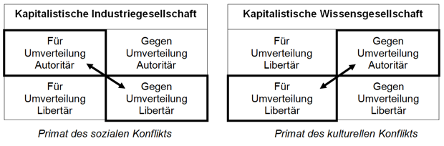
\includegraphics[width=\textwidth,height=\textheight,keepaspectratio]{../Bilder/brie2.png} 
\end{figure*}

    Kitschelt und Rehm nehmen die folgenden Einstellungen als Maßstab, um libertäre von autoritären Orientierungen zu unterscheiden: Es ginge dabei um „nichtökonomische Fragen der bürgerlichen Freiheiten und der Rechtsordnung, um Geschlechterrollen und sexuelle Orientierung, um die unhinterfragte Einhaltung kollektiver Normen,\endnote{Eigentlich müsste es heißen: „um die Ablehnung der unhinterfragten Einhaltung kollektiver Normen“, da alle Formulierungen libertäre Einstellung im Sinne von Kitschelt und Rehm implizieren.}  um die Toleranz gegenüber kultureller Vielfalt von Überzeugungen und Praktiken sowie unterschiedlichen Lebensstilen und um die Akzeptanz der Einwanderung aus Gesellschaften mit anderen kulturellen Bräuchen“ (Kitschelt, Rehm 2022: 4). Libertäre Einstellungen werden daran festgemacht, dass die jeweilige Person die Legalisierung der Heirat von Personen gleichen Geschlechts befürwortet, sie sich für private Rechte auch dann einsetzt, wenn dies die Bekämpfung von Kriminalität behindert, sie gegen eine restriktive Einwanderungspolitik ist und den Umweltschutz auch dann einfordert, wenn er das Wirtschaftswachstum einschränkt, und wenn sie eine weitere Europäisierung fordert (ebd.: 38). 

Die Schwierigkeiten der Klassifikation libertär/ autoritär werden dann deutlich, wenn man unter dem Aspekt des Umweltschutzes die Forderungen nach der gesetzlichen Einschränkung des Fleischkonsums, die Einführung eines Tempolimits auf Autobahnen oder das Verbot des Tragens eines Kopftuchs durch Lehrerinnen in Schulen hinzuzieht. In jedem dieser Fälle würden eindeutig Freiheiten der Einzelnen eingeschränkt. Die gleichen Personen, die dem Zuzug „aus anderen Kulturen“ offen gegenüberstehen, können zugleich verlangen, dass diese die in ihren Herkunftsländern üblichen Symbole nicht öffentlich zeigen, weil ihnen unterstellt wird, damit „autoritäre“ Werte zu propagieren, und dies selbst dann, wenn die Trägerinnen eines Kopftuchs dies genau umgekehrt als Zeichen des Selbstbewusstseins der eigenen Identität gegenüber einer „westlichen“ Umwelt verstehen können. Die Freiheitsrechte der Einzelnen unterliegen bei den von Kitschelt und Rehm verwandten Kriterien offensichtlich einer Zensur, wobei es libertär sein soll, möglichst wenige Freiheitsrechte einzuschränken, wenn es um Kriminalität geht, aber möglichst viele, wenn es um Umweltschutz geht. Die „libertären“ Grünen waren Vorreiter der Beschränkungen vieler Freiheitsrechte in der Corona-Pandemie, während die „autoritäre“ AfD sich vehement dagegen aussprach. Die scheinbar wertneutrale Klassifikation erweist sich bei näherer Betrachtung als zutiefst ambivalent: Freiheiten der Einzelnen werden je nach Bezug auf bestimmte gemeinschaftliche Orientierungen (Umweltschutz, offene Gesellschaft, westlich-liberales kulturelles Selbstverständnis) entweder positiv als „libertär“ auf- oder negativ als „autoritär“ abgewertet.

Auch der Begriff „autoritär“ erweist sich bei näherem Hinsehen als zutiefst ambivalent. Anders als der Begriff libertär ist der Begriff des Autoritären historisch dezidiert negativ konnotiert. Er wird im direkten Gegensatz zu dem der Freiheit gesehen. Nach diesem Verständnis ist Freiheit im Sinne von Isaiah Berlin die Freiheit von Eingriffen anderer Menschen oder Gruppen von Menschen in das Handeln der Einzelnen (Berlin 2006: 201) und damit die Möglichkeit, von anderen unabhängige Entscheidungen zu treffen. Berlin unterscheidet von der negativen Freiheit die positive Freiheit, die auf die Frage antwortet: „Von was oder von wem geht die Kontrolle oder die Einmischung aus, die jemanden dazu bringen kann, dieses zu tun oder zu sein und nicht jenes andere?“ (Ebd.) 

Wieso aber sollte es autoritär, sprich: fremdbestimmt sein, negative Freiheiten der Einzelnen auf der Basis gemeinsamer Beschlüsse einzuschränken, wenn es um Kriminalität geht, aber Ausdruck libertärer, sprich: freiheitlicher Einstellungen, wenn es sich um Einschränkungen jener individuellen Freiheiten handelt, die den Umweltschutz betreffen? Wieso wird es als libertär angesehen, weitgehende Zuzugsrechte für Ausländer zu fordern, aber als autoritär, wenn gefragt wird, ob damit nicht unter den konkreten Bedingungen heutiger Gesellschaften Freiheits- und Schutzrechte von Inländern bedroht sind? Die Linke zumindest kann doch nicht blind dafür sein, dass Globalisierung die Konkurrenz zwischen verschiedenen Gruppen der Lohnarbeitenden verschärft hat und die Grenzen unter kapitalistischen Bedingungen zwangsläufig die Funktion haben, der Regulation dieser Konkurrenz zu dienen. Um den Charakter dieser Regulation muss zwangsläufig gekämpft werden.

Die Ambivalenz des Begriffs des Autoritären wird deutlich, wenn man auf die bekannten „Studien über Autorität und Familie“ des Instituts für Sozialforschung von 1936, damals schon im Exil in den USA, zurückgreift. Im allgemeinen Teil zur Einführung in diese Studien schrieb Max Horkheimer: „Wenn wir vorläufig als autoritär jene inneren und äußeren Handlungsweisen ansehen, in denen sich die Menschen einer fremden Instanz unterwerfen, so springt sogleich der widerspruchsvolle Charakter dieser Kategorie in die Augen. Das autoritäre Handeln kann im wirklichen und bewussten Interesse von Individuen und Gruppen liegen.“ (Horkheimer 1987: 24) Er macht auf den historisch-konkreten progressiven Charakter bestimmter Formen von Autorität in Familie und Gesellschaft aufmerksam und schreibt: „[…] ob die bedingungslose Unterordnung unter einen politischen Führer oder eine Partei historisch nach vorwärts oder rückwärts weist, vermag allein die Analyse der jeweiligen gesellschaftlichen Situation in ihrer Totalitat zu beantworten“ (ebd.: 25). Gegen naive libertäre Vorstellungen vom Segen einer unbegrenzten negativen Freiheit der Einzelnen ist Horkheimers folgende Beobachtung gerichtet: „Die Lockerung von Abhängigkeits-Verhältnissen, welche im bewussten und unbewussten Leben der Masse verwurzelt sind, gehört zu den größten Gefahren für eine bestehende gesellschaftliche Struktur und zeigt an, dass sie spröde geworden ist.“ (ebd.: 26) Die Überhöhung der negativen Freiheit der Einzelnen zur Freiheit schlechthin steht für Marx wie Horkheimer unter dem gut begründeten Verdacht, „eine Ideologie“ zu sein, „das heißt ein durch die spezifische Form des gesellschaftlichen Lebensprozesses notwendig bedingter Schein“ (ebd.: 41).

Wieso aber unterwerfen sich Menschen, folgt man Horkheimers Bestimmung von „autoritär“, überhaupt einer „fremden Instanz“, wenn deren Vorgaben „im wirklichen und bewussten Interesse von Individuen und Gruppen liegen“?  In diesem Falle wären es doch die eigenen Interessen? Was in dieser Formulierung unreflektiert aufscheint, ist die tiefe Spannung der Interessen der vielen Einzelnen als Einzelne und als Mitglieder eines Gemeinwesens. Es war Rousseau, der dies ins Zentrum seiner Sozialphilosophie rückte. In der Schrift „Vom Gesellschaftsvertrag“ heißt es: „Oft besteht ein großer Unterschied zwischen dem Willen aller (volonté de tous) und dem Gemeinwillen (volonté générale); letzterer zielt nur auf das Gemeininteresse (l'intérêt commun), ersterer auf das Einzelinteresse (l'intérêt privé) und ist nur die Summe von Einzelwillen (somme de volontés particulières)“ (Rousseau 1989: 403). Damit deckte Rousseau eine unleugbare Tatsache auf: Zwei Seelen wohnen in der Brust eines jeden, der in einer komplexen Gesellschaft lebt, in der die Reproduktion der unmittelbaren Gemeinschaftsbeziehungen und die des Gesellschaftskörpers auseinanderfallen. Hegel hat dies als Gegensatz von Bourgeois und Citoyen aufgegriffen (Hegel 1981: 224-226, § 187), dem bei ihm der eigentumslose „Pöbel“, das Proletariat, als fremd entgegensteht (Ruda 2011), da es keine Allgemeininteressen haben könne. 

Bei Freud wurde die Spannung zwischen dem Individuum als Einzelner und als Gesellschaftsglied psychoanalytisch als Unterscheidung von „Es“ und „Über-Ich“ aufgenommen. Diese Spannung stelle dem „Ich“ die Aufgabe, zwischen beiden zu vermitteln und sie in ein lebensfähiges Verhältnis zu bringen. Fromm schrieb dazu: „Durch das Über-Ich wird die äußere Gewalt transformiert und zwar, indem sie aus einer äußeren in eine innere Gewalt verwandelt wird. Die Autoritäten als die Vertreter der äußeren Gewalt werden verinnerlicht, und das Individuum handelt ihren Geboten und Verboten entsprechend nun nicht mehr allein aus Furcht vor äußeren Strafen, sondern aus Furcht vor der psychischen Instanz, die es in sich selbst aufgerichtet hat.“ (Fromm 1987: 84) Kant paraphrasierend könnte man auch sagen, dass Menschen gar nicht umhin können, in sich ein autoritatives Sittengesetz zu verankern, wenn sie autonom handeln wollen. Die Frage ist nur, für welches Sittengesetz sie sich entscheiden. Wirkliche Freiheit und Autonomie einerseits und verinnerlichte Autoritäten andererseits bilden einen Gegensatz, dem nur um den Preis der Verdrängung ins Unterbewusstsein und damit aus dem Reich bewusster Reflexion ausgewichen werden kann. Alles dies verbietet eine naive Verurteilung von Autorität.

Der Terminus autoritär verschmilzt bei Kitschelt und Rehm, wie aber auch insgesamt in großen Teilen der Parteienforschung, die auf die genannten Befragungen zurückgreifen, unterschiedliche Positionen. Es werden die Werte von Gemeinschaftlichkeit (im Sinne einer In-Group-Orientierung), der Einhaltung von Gruppenregeln, des Anspruchs auf Schutz als Teil einer Gruppe einerseits mit Positionen der gruppenbezogenen Menschenfeindlichkeit (Heitmeyer 2010) oder eines „autoritären Charakters“ im Sinne von Erich Fromm andererseits in eins gesetzt. Fromm hatte den autoritären Charakter so definiert: „Wenn mangelnde Fähigkeit zum selbständigen Handeln die Einstellung des autoritären Charakters zum Stärkeren kennzeichnet, so bietet seine Einstellung zum Schwächeren und Hilflosen eine Kompensation. Ebenso automatisch wie Macht in ihm Furcht und, wenn auch ambivalente, Liebe erweckt, erweckt Hilflosigkeit in ihm Verachtung und Hass.“ (Fromm 1987: 116.) Gerade das Kleinbürgertum sei dafür empfänglich (Fromm 2000: 203). 

Um es drastisch auszudrücken: Eine Verwendung des Terminus „autoritär“, der die genannte Differenz zwischen Gemeinschaftsorientierungen und gruppenbezogener Menschenfeindlichkeit einebnet, tendiert dazu, alle jene, die aufgrund der geringeren Chancen auf dem Arbeitsmarkt („geringe Bildung“) und eines niedrigeren sozialen Erfolgs („niedriges Einkommen“) gleichzeitig soziale Umverteilung und Schutz durch Staat und Gesellschaft vor dem ungehinderten Wirken der Konkurrenzverhältnisse der Märkte fordern, zu verachten und, schlimmer noch, als „braune Dumpfbacken“ abzutun, die auf dem besten Wege in den rassistischen National-Sozialismus sind oder dort schon angekommen. Wenn die Linke dem folgt und diese Gruppen als Pöbel aufgibt (so sehr plastisch und nachdrücklich Baron 2016), hat sie jede Chance auf Gegen-Hegemonie und einen eigenständigen „Dritten Pol“ (Candeias 2016) jenseits des Sozialliberalismus und der Neuen Rechten vertan. Es ist das eine, in den Enklaven der gehobenen Mittelschichten in den Metropolregionen die uneingeschränkte Freiheit der Einzelnen zu zelebrieren, es ist etwas anderes, in Gebieten mit weit höherer Kriminalität und Gewalt zu leben. Es ist das eine, den Zuzug billiger Servicekräfte für die oberen Mittelschichten zu begünstigen, es ist das andere, mit diesen Neumigranten auf dem leergefegten Markt für preiswerte Wohnungen zu konkurrieren.

Während die Achse Soziale Umverteilung vs. Stärkung der Märkte auf der Ebene der Instrumente argumentiert, mit denen sehr unterschiedliche Werte verfolgt werden können,\endnote{Die Stärkung bestimmter Märkte und des Wettbewerbs auf ihnen kann durchaus in bestimmten Fällen soziale Gleichheit befördern und z. B. patriarchale Strukturen abzubauen helfen, wie u. a. Nancy Fraser (2015: 110f.) nachwies. Sie kann auch gegen Gruppen der Kapitaloligarchien und ihrer Hauptvertreter gerichtet sein.}  werden auf der Achse Libertär vs. Autoritär von Kitschelt und Rehm wie vielen anderen Wertbegriffe benutzt, die in ihrer Widersprüchlichkeit nicht reflektiert werden. Dadurch wird die von Max Weber erhobene Forderung nach der Wertfreiheit der wissenschaftlichen Instrumente bei gleichzeitiger Transparenz des Wertbezugs des Ziels der Forschungen verletzt (Weber 1922). Die Forschung schafft damit im konkreten Fall nicht den Raum der analytischen Reflexion von wertenden Differenzen im politischen Spektrum, sondern dupliziert die vorhandenen Klassifikationen jener, die für sich das Epitheton libertär als positive Selbstbezeichnung reklamieren.

\section{Wieso es so schwer ist, eine solidarische Linke zu formieren}

\noindent Wenn man analog zur horizontalen Konfliktlinie Soziale Umverteilung vs. Marktkonkurrenz auch die vertikale Konfliktlinie nicht unmittelbar über Werte, sondern über gesellschaftliche Mittel definieren würde, mit denen unterschiedliche Ziele verfolgt werden können, dann scheint es sinnvoll, die Kategorie libertär durch die des Primats individueller Freiheit im Sinne von negativer Freiheit der Einzelnen (Berlin 2006) zu ersetzen. Es geht um die Stärkung der Rechte der Individuen, ausschließlich aus eigenem Ermessen heraus frei zu entscheiden. Anstelle der Kategorie autoritär würde, folgte man diesem Vorschlag, das Primat der Orientierung an gemeinschaftlichen Zielen verwandt werden. Dies erlaubt es, vier grundlegende ideologische Orientierungen zu unterscheiden – die soziallibertäre, die marktliberale, die sozialpopuläre und die marktkonservative Orientierung (Abb. 3).

\begin{figure*}
    \centering
    \caption{Politische Projekte}
    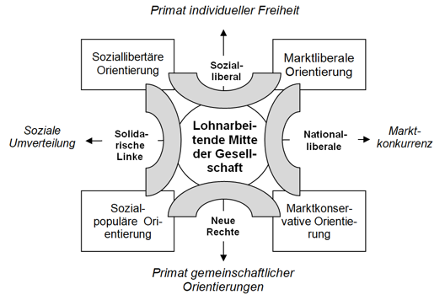
\includegraphics[scale=0.8]{../Bilder/brie3.png} 
\end{figure*}

Wer Gegen-Hegemonie anstrebt, muss danach streben, die vorhandenen hegemonialen Verknüpfungen aufzulösen und die Elemente wieder frei setzen, um sie in Momente neuer Verbindungen zu verwandeln (Laclau, Mouffe 2000: 143). Die zentralen politischen Projekte, die sich heute gegenüberstehen, sind nicht zufällig Projekte der Verbindung zweier sehr unterschiedlicher ideologischer Orientierungen, wie Grafik 3 verdeutlicht. Anders würden sie auch nicht mehrheitsfähig sind können. In der Bundesrepublik dominiert gegenwärtig das sozialliberale Projekt, dass in der Ampel-Regierung seinen geradezu idealtypischen Ausdruck gefunden hat. Ihm steht mit der AfD eine Neue Rechte gegenüber als dem zweiten Pol. Weder die Nationalliberale noch eine Solidarische Linke vermochten bisher einen wirksamen Dritten Pol bilden. Das nationalliberale Projekt scheiterte mit der frühen AfD und Bernd Lucke, das Projekt einer solidarischen Linken droht im politischen Raum mit der Partei DIE LINKE zu scheitern.

Eine solidarische Linke kann sich nur dann erfolgreich formieren, wenn es ihr gelingt, eine Reihe von Aufgaben zu erfüllen. Die erste Aufgabe ist die, bei Hegel in die Schule zu gehen. Es ist kein Zufall, dass wirkungsstarke linke Politiker des 20. Jahrhunderts wie Lenin, Mao Zedong oder Gramsci sich intensiv mit der Hegelschen Dialektik auseinandergesetzt haben – sei es direkt oder wie bei Mao Zedong über Lenin, der am Beginn des Ersten Weltkriegs in die Berner Bibliothek ging und vier Monate lang Hegels „Wissenschaft der Logik“ studierte (siehe ausführlicher Brie 2017: 19-24). Linke Politik ist immer Segeln gegen den Wind der herrschaftlichen Verhältnisse, ist immer mit deren Tendenz der Spaltung der subalternen Klassen im Sinne von divide et impera konfrontiert. Am „Rande des Abgrunds“ (Gagnebin 2011: 285; siehe im Detail Eiland, Jennings 2020: 866-872) und konfrontiert mit den entgegenstürmenden Gewalten von Krieg, Judenverfolgung und dem Nichtangriffsvertrag zwischen Deutschland und der Sowjetunion schrieb Walter Benjamin im Spätwinter 1939/40: „Dialektiker sein heißt den Wind der Geschichte in den Segeln zu haben. Die Segel sind die Begriffe. Es genügt aber nicht, über die Segel zu verfügen. Die Kunst, sie setzen zu können, [um gegen den Sturm anzukreuzen – M. B.] ist das Entscheidende.“ (Benjamin 1982: 592) Nimmt man das stromlinienförmige Schiff mit seinem Kiel und dem Steuer als Metapher für eine handlungsfähige Organisation und die richtig gesetzten Segel als Symbol von Führungsfähigkeit, wird deutlich, was es heißt, die Widersprüche der Herrschaft zum Zwecke ihrer Überwindung zu nutzen. Diese Kunst haben offensichtlich viele linke Kräfte verlernt oder schlicht nie gelernt. 

Viel zu viel linke Politik erschöpft sich in gut gemeinter Realpolitik einerseits oder in noch besser gemeinter Verfolgung reiner Ideale andererseits. Eine die Herrschaftsverhältnisse transformierende und überwindende „revolutionäre Realpolitik“ (Luxemburg 1979: 373) ist auf diese Weise unmöglich. Diese verlangt, sich auf die realen Widersprüche einzulassen und sie zugleich gegenhegemonial, gegenherrschaftlich zu nutzen. Dies zumindest kann man bei Lenin lernen, der im Zusammenhang mit dem bewaffneten Osteraufstand in Irland 1916 schrieb: „[…] zu glauben, dass die soziale Revolution denkbar ist ohne Aufstände kleiner Nationen in den Kolonien und in Europa, ohne revolutionäre Ausbrüche eines Teils des Kleinbürgertums mit allen seinen Vorurteilen, ohne die Bewegung unaufgeklärter proletarischer und halbproletarischer Massen gegen das Joch der Gutsbesitzer und der Kirche, gegen die monarchistische, nationale usw. Unterdrückung – das zu glauben heißt der sozialen Revolution entsagen. […] Wer eine ›reine‹ soziale Revolution erwartet, der wird sie niemals erleben. Der ist nur in Worten ein Revolutionär, der versteht nicht die wirkliche Revolution.“ (Lenin 1971: 363, 364.)

Eine zweite Aufgabe besteht darin, die Überzeugung in größeren Teilen der Gesellschaft zu verankern, dass es eine wirkliche Alternative zum Kapitalismus gibt, der seit mehr als einem Jahrzehnt die Gesellschaften mit einer schweren Krise nach der anderen überzieht und jetzt in den Dauermodus eines Krisen- und Kriegskapitalismus übergegangen ist. Es ist im Zeitalter des neuen Krisen-, Katastrophen- und Kriegskapitalismus kein Zufall, dass eine neue Sozialismusdiskussion in den politisch-öffentlichen Raum drängt. Die Zeit des Verstummens nach dem „seltsamen Tod des Sozialismus“ (Dahrendorf 1990) ist vorbei. Im Mai 2022 erhielt ich die Nachricht: „41.613 neue Arbeiten zum Thema 'Theorien des Sozialismus' wurden seit Ihrer letzten Suche in Academia veröffentlicht.“ Auch wenn tatsächlich diese Suche mehrere Jahre zurückliegt, ist die Zahl doch bemerkenswert. Der Neoliberalismus konnte das vom Marxismus-Leninismus hinterlassene Vakuum nicht lange füllen. Jüngst sind immer neue Bücher und Grundsatzartikel erschienen, die die Frage nach Sozialismus ins Zentrum rücken. Nicht nur international, sondern auch im überschaubaren deutschsprachigen Raum gibt es eine ganze Serie von Publikationen zum Sozialismus (Crome 2006; Dellheim u. a. 2012; Paech 2012; Klein 2013; Honneth 2015; Winker 2015; Dörre, Schickert 2019; Zelik 2020; Zeller 2020; Dörre 2021; Klein 2022).

Eine sozialistische Alternative muss heute anders als in der Vergangenheit in sich das Erbe von Liberalismus und Kommunismus aufnehmen (zu den sehr wenigen, die dies ausgehend von den Erfahrungen des Faschismus und Stalinismus anstrebten, gehört Ernst Bloch 2007). Es gibt einerseits den Kampf des Liberalismus für persönliche Autonomie und Überwindung der Abhängigkeit von vorgefundenen Herrschaftsformen. Es geht um individuelle Freiheitsrechte und Handlungsmöglichkeiten, um die Chance Einzelner, etwas Neues zu wagen, auch gegen heftigste Widerstände. Die Gestaltung von Wirtschaft und Politik ausgehend von der freien Initiative der Einzelnen und ihren selbstbestimmten Zusammenschlüssen steht im Zentrum. Dies war und ist zugleich ein Kampf gegen den Kommunismus der Allmende, der Gemeingüter und ihrer Verteilung nach den Bedürfnissen. Diese Gemeingüter und die gemeinschaftliche Regulierung der Verfügung über sie wurden als Hindernisse auf dem Weg zu einer offenen Gesellschaft der Freien gesehen. Es gibt andererseits den Kampf des Kommunismus gegen die Ausbeutungsstrukturen, die mit dem kapitalistischen Privateigentum verbunden sind, und um die Bewahrung der Gemeingüter – der natürlichen wie der sozialen und kulturellen, ein Kampf um jene Gemeinschaftsformen, die Freiheit und Gleichheit substantiell zu begründen vermögen. Dies war und ist auch ein Kampf gegen die Vorherrschaft privater Rechte und des Privateigentums und für die gemeinsame Kontrolle über die Produktions- und Reproduktionsmittel. In ein neues Verständnis von Sozialismus muss überzeugend beides eingehen – die Betonung der Freiheitsrechte der Einzelnen und der Kampf um die Gemeingüter eines Lebens in Solidarität.

Sozialismus sollte als eine Gesellschaft verstanden werden, die sich erstens ihrer kommunistischen Fundamente bewusst ist und diese verantwortungsvoll bewahrt und stärkt, sich zweitens an den Werten von Freiheit, Gleichheit und Solidarität ausrichtet und drittens Menschen ermöglicht, ein erfülltes Leben zu führen. Dies alles ist nur möglich, wenn eine solche Gesellschaft über wirksame Akteure und Institutionen verfügt, die diese dreifache Aufgabe erfüllen. Sozialismus ist, folgt man diesem Verständnis, jene Bewegungsform der Widersprüche komplexer moderner Gesellschaft, die in der Lage ist, Ausbeutung, Unterdrückung und Entmündigung von Menschen durch Menschen und Ausbeutung der Natur hinter sich zu lassen. Als solche stellt Sozialismus tatsächlich den überlebenswichtigen Weg dar, der über Liberalismus und Kommunismus hinausgeht. Die kommunistischen Fundamente bilden die gemeinsame „Erde“ dieser Gesellschaft; Freiheit, Gleichheit und Solidarität die Fixsterne am „Himmel“; und die Akteure und Institutionen des Sozialismus sollten die Fähigkeit entwickeln, zwischen diesem Himmel und dieser Erde zu vermitteln. Jede und jeder erhalten damit die Chance, ein erfülltes, reiches Leben zu führen. Sozialismus kann dafür nur die Möglichkeiten schaffen, einlösen müssen die Menschen diese Möglichkeiten selbst. 

Die dritte Aufgabe bei der Gründung einer solidarischen Linken ist die Arbeit an einem neuen klassenverbindenden Bündnis (Candeias 2017). Der Siegeszug des neoliberalen Finanzmarkt-Kapitalismus war nur möglich, weil er verhindern konnte, dass die mit der „Wissensgesellschaft“ aufstrebenden neuen Gruppen mit höherer Bildung ein Bündnis mit der „alten“ organisierten Arbeiterbewegung eingingen. Die Herrschenden betrieben erfolgreich Klassenspaltung. Der Neoliberalismus konnte deshalb hegemonial werden, weil er die Freiheitsansprüche neuer sozialer Schichten und Generationen mit dem Projekt des Umbaus des Sozialstaats in den Wettbewerbsstaat einer den Interessen der Kapitaloligarchien untergeordneten Globalisierung zu verbinden vermochte. Die Entfesselung der Märkte wurde zum Freiheitsversprechen gemacht. Die soziale Frage wurde durch die Frage der Freiheit der Individuen, der Unternehmen, der Erfolgreichen abgelöst. Anstelle sozialer Bindung wurde der Kult der Freiheit der Einzelnen ins Zentrum gerückt (Boltanski, Chiapello 2003). Wenn die Linke zu einem eigenen „Dritten Pol“ werden will, der die Kräfteverhältnisse umzugestalten vermag, dann müsste es ihr gelingen, die Dominanz des Konflikts zwischen individuellem Freiheitsversprechen und Gemeinschaftsorientierung (die vertikale Konfliktachse) zu überwinden und die horizontale Konfliktachse wieder ins Zentrum der gesellschaftspolitischen Auseinandersetzungen zurück zu rücken. Es geht um eine materialistische Wendung, die auch das Kulturelle als Ausdruck der realen gesellschaftlichen Praxis und der in ihnen eingeschriebenen sozialen Ungleichheits- und Ausbeutungsverhältnisse begreift.

\section{Über das Interregnum hinaus}

\noindent Dies wäre kein Zurück zur Vergangenheit, sondern dialektische Aufhebung des jetzigen Großkonflikts, indem die erzielten Freiheitsgewinne, die gewachsene Bedeutung von Fragen des Geschlechts und der sexuellen Orientierung, der Ethnie und Herkunft integriert werden in eine neue Politik der sozialen Gerechtigkeit, die den dezidierten Schutz der Schwachen, die Sensibilität für die transnationalen Dimensionen der Ungleichheit, die sozialökologische Umgestaltung der Gesellschaft, Wirtschaftsdemokratie, inklusive Städte und Regionen für alle und partizipatorische Demokratie miteinander verbinden (Dörre 2021; Winker 2021; Fraser 2022) und auch die dafür notwendige Regulationsweise und demokratischen Formen entwickeln (Klein 2022).

Dies ist aber nur möglich, wenn es der Linken gelingt, die liberale Identifikation von gruppenbezogener Menschenfeindlichkeit einerseits mit Orientierungen an gemeinschaftlichen Werten und Lebensformen andererseits aufzubrechen. Es ist diese Konstruktion, die in das generalisierte Feindbild des „Autoritären“ und des „Autoritarismus“ mündete. Umgekehrt muss die Linke die Reduktion von Freiheit auf die negative Freiheit der Individuen angreifen, die das heutige Bündnis von „grünen“ und „libertären“ Parteien mit den Kräften der Marktfreiheit begründet. Bei Freiheit geht es auch um die gemeinsame Entscheidung darüber, wie ein Gemeinwesen gestaltet wird. Freiheit kann, um noch einmal auf Isaiah Berlin zu verweisen, auch die Freiheit sein, positiv zu entscheiden, was in einer Gesellschaft geboten ist. Und außerdem geht es immer darum, wie diese Freiheit genutzt wird, welche Substanz sie hat, welche Ziele verfolgt werden, welche Gesellschafts- und Lebensentwürfe verfolgt werden. Eine neue Dominanz des Sozialen in den gesellschaftspolitischen Kämpfen braucht einen neuen Begriff von Freiheit, der mehrdimensional ist (Brie 2016).

Konkret wird eine solche die Lohnarbeitenden verbindende Politik dann, wenn verbindende Einstiegsprojekte (Brangsch 2014; Institut für Gesellschaftsanalyse \& Friends 2020) entwickelt werden. Erfolge dabei zeigten sich in der Wohnungsfrage und bei Forderungen eines ÖPNV, bei dem die Fahrentgelte sehr gering sind, wie das Neun-Euro-Ticket zeigte. Es eröffnete Geringverdienern und Einkommensschwachen wieder den Zugang zur eigenen Stadt und dem Umland und war zugleich ökologisch. Auch die Forderung nach einer sehr preiswerten Grundversorgung mit Wasser und Energie bzw. die Schaffung von Jobs im Bereich des sozialökologischen Umbaus gehören dazu. Alle diese Forderungen werden gerade von denen mit niedrigem Einkommen besonders unterstützt (Arbeitsgruppe des Vorstands der Rosa-Luxemburg-Stiftung 2022: 23).

Alle philosophische Dialektik, alle Arbeit an neuen Alternativvorstellungen, alle Bemühungen, solidarische Einstiegsprojekte zu entwickeln, reichen aber nicht. Ideen müssen viertens Organisation werden, wenn sie wirken sollen. Ein linkes Mosaik (Urban 2009) zerbricht schnell an jedem Konflikt. Besonders im politischen Raum fehlt in fast allen westlichen Ländern eine starke linke politische Kraft. Die Projekte von Sanders und Corbyn scheiterten vorerst. Das von Jean-Luc Mélenchon geführte Bündnis NUPES (Nouvelle union populaire écologique et sociale) muss sich erst noch bewähren. Ohne festen Halt im politischen System können soziale Bewegungen nicht über Achtungserfolge hinauskommen und Gewerkschaften haben keinen Partner für eine wirklichen Politikwechsel.

Ein Blick auf die vier genannten Aufgaben begründet, warum es im parteipolitischen Raum so schwierig ist, eine erfolgreiche Repräsentanz einer solidarischen, die Lohnarbeitenden verbindenden Linken aufzubauen. Angesichts der Fundamentalkrise der heutigen kapitalistischen Gesellschaften muss dies aber nicht so bleiben. Solche organischen Krisen erzeugen ein Interregnum (Gramsci 1992: 493f.) und dies sind Zeiten von Aufbrüchen, wenn auch mit ungewissem Ausgang. Aber sie können auch, wie schon in der Geschichte, zu Zeiten einer neuen, einer solidarischen Linken werden.



    \printendnotes[custom]
    
\section{Literatur}
    \begin{bibdescription}
        \item Arbeitsgruppe des Vorstands der Rosa-Luxemburg-Stiftung (2022): Eine starke Partei DIE LINKE ist möglich und wird gebraucht! Zehn Herausforderungen für einen solidarischen Aufbruch. URL: https://www.rosalux.de/fileadmin/rls\_uploads/pdfs/sonst\_publikationen/Broschur\_Eine\_starke\_Partei\_DIE\_LINKE\_Web2.pdf. 
        \item Baron, Christian (2016): Proleten, Pöbel, Parasiten. Warum die Linken die Arbeiter verachten. Berlin: Das Neue Berlin.
        \item Benjamin, Walter (1982): Das Passagen-Werk. In: Gesammelte Schriften, Bd. V. Frankfurt a. M.: Suhrkamp.
        \item Berlin, Isaiah (2006): Freiheit. Vier Versuche. Frankfurt a. M.: Fischer Taschenbuch.
        \item Bloch, Ernst (2007): Naturrecht und menschliche Würde. Frankfurt a. M.: Suhrkamp.
        \item Boltanski, Luc; Chiapello, Ève (2003): Der neue Geist des Kapitalismus. Konstanz: UVK.
        \item Brangsch, Lutz (2014): Transformationsprozesse und ihre Politisierung in Einstiegsprojekten. In: Brie, Michael (Hrsg.): Futuring. Transformation im Kapitalismus über ihn hinaus. Münster: Westfälisches Dampfboot, S. 368-391.
        \item  Brie, Michael (2016): Emanzipation – eine Vier-in-Einem-Perspektive. Ein Diskussionsvorschlag. Ms.
        \item Brie, Michael (2017): Lenin neu entdecken: Das hellblaue Bändchen zur Dialektik der Revolution \& Metaphysik der Herrschaft. Hamburg: VSA.
        \item Candeias, Mario (2016): Den „dritten Pol“ wieder sichtbar machen. In: Neues Deutschland, 22. April 2016. URL: https://www.neues-deutschland.de/artikel/1009532.den-dritten-pol-wieder-sichtbar-machen.html.
        \item Candeias, Mario (2017): Eine Frage der Klasse. Neue Klassenpolitik als verbindender Antagonismus. In: LuXemburg. Gesellschaftsanalyse und linke Praxis (Sonderausgabe).
        \item Crome, Erhard (2006): Sozialismus im 21. Jahrhundert. Zwölf Essays über die Zukunft. Berlin: Karl Dietz.
        \item Dahrendorf, Ralf (1990): The Strange Death of Socialism. In: An Irish Quarterly Review 79, S. 7-17.
        \item Dellheim, Judith; Brangsch, Lutz; Wolf, Frieder-Otto; Spangenberg, Joachim (2012): Den Krisen entkommen. Sozialökologische Transformation. Berlin: Karl Dietz.
        \item Dörre, Klaus (2021): Die Utopie des Sozialismus. Kompass für eine Nachhaltigkeitsrevolution. Berlin: Matthes \& Seitz.
        \item Dörre, Klaus; Schickert, Christiane (Hrsg.) (2019): Neosozialismus: Solidarität, Demokratie und Ökologie vs. Kapitalismus. München: oekom.
        \item Eiland, Howard; Jennings, Michael W. (2020): Walter Benjamin. Eine Biographie. Berlin: Suhrkamp.
        \item Fraser, Nancy (2015): Dreifachbewegung. Die politische Grammatik der Krise nach Karl Polanyi. In: Brie, Michael (Hrsg.): Polanyi neu entdecken. Das hellblaue Bändchen zu einem möglichen Dialog von Nancy Fraser \& Karl Polanyi. Hamburg: VSA, S. 100-116.
        \item Fraser, Nancy (2022): Cannibal Capitalism. How Our System Is Devouring Democracy, Care, and the Planet and What We Can Do About It. New York: Verso.
        \item Fromm, Erich (1987): Sozialpsychologischer Teil. In: Horkheimer, Max (Hrsg.): Studien über Autorität und Familie. Forschungsberichte aus dem Institut für Sozialforschung. Reprint der Ausgabe Paris 1936. Lüneburg: zu Klampen Verlag, S. 77-135.
        \item Fromm, Erich (2000): Die Furcht vor der Freiheit. München: dtv.
        \item Gagnebin, Jeanne Marie (2011): „Über den Begriff der Geschichte“. In: Lindner, Burkhardt (Hrsg.): Benjamin Handbuch. Leben – Werk – Wirkung. Stuttgart: Metzler, S. 284-300.
        \item Gramsci, Antonio (1992): Gefängnishefte. Kritische Gesamtausgabe. Bd. 3. Heft 4-5. Hamburg: Argument.
        \item Hegel, Georg Wilhelm Friedrich (1981): Grundlinien der Philosophie des Rechts oder Naturrecht und Staatswissenschaft im Grundrisse. Nach der Ausgabe von Eduard Gans. Herausgegeben und mit einem Anhang versehen von Hermann Klenner. Berlin: Akademie Verlag.
        \item Heitmeyer, Wilhelm (2010): Deutsche Zustände. Frankfurt a. M.: Suhrkamp.
        \item Honneth, Axel (2015): Die Idee des Sozialismus. Versuch einer Aktualisierung. Berlin: Suhrkamp.
        \item Horkheimer, Max (1987): Allgemeiner Teil. In: Ders (Hrsg.): Studien über Autorität und Familie. Forschungsberichte aus dem Institut für Sozialforschung. Reprint der Ausgabe Paris 1936. Lüneburg: zu Klampen Verlag, S. 3-76.
        \item Institut für Gesellschaftsanalyse \& Friends (2020): Ein Gelegenheitsfenster für linke Politik? Wie weiter in und nach der Corona-Krise. URL: https://zeitschrift-luxemburg.de/artikel/ein-gelegenheitsfenster-fuer-linke-politik-wie-weiter-in-und-nach-der-corona-krise/.
        \item Kitschelt, Herbert P.; Rehm, Philipp (2022): Polarity Reversal: The Socioeconomic Reconfiguration of Partisan Support in Knowledge Societies. In: Politics \& Society, S. 1-47.
        \item Klein, Dieter (2013): Das Morgen tanzt im Heute. Transformation im Kapitalismus und über ihn hinaus. Hamburg: VSA.
        \item  Klein, Dieter (2022): Regulation in einer solidarischen Gesellschaft. Wie eine sozial-ökologische Transformation funktionieren könnte. Hamburg: VSA.
        \item Laclau, Ernesto; Mouffe, Chantal (2000): Hegemonie und radikale Demokratie. Zur Dekonstruktion des Marxismus. Wien: Passagen.
        \item Lenin, Wladimir I. (1971): Die Ergebnisse der Diskussion über die Selbstbestimmung. In: Werke, Bd. 22. Berlin: Dietz, S. 326-368.
        \item Luxemburg, Rosa (1979): Karl Marx (1903). In: Gesammelte Werke, Bd. 1.2. Berlin: Dietz, S. 369-377.
        \item Paech, Niko (2012): Befreiung vom Überfluss. Auf dem Weg in die Postwachstumsökonomie. München: Oekom.
        \item Rousseau, Jean-Jacques (1989): Vom Gesellschaftsvertrag oder Prinzipien des Staatsrechts. In: Kulturkritische und politische Schriften in zwei Bänden. Bd. 1. Berlin: Rütten \& Loening, S. 379-505, 635-648.
        \item Ruda, Frank (2011): Hegels Pöbel. Eine Untersuchung der „Grundlinien der Philosophie des Rechts“. Konstanz: Konstanz University Press.
        \item Urban, Hans-Jürgen (2009): Die Mosaik-Linke. Vom Aufbruch der Gewerkschaften zur Erneuerung der Bewegung. In: Blätter für deutsche und internationale Politik, H. 5, S. 71-77.
        \item Weber, Max (1922): Wissenschaft als Beruf (1919). In: Gesammelte Aufsätze zur Wissenschaftslehre. Tübingen: Mohr, S. 524-555.
        \item Winker, Gabriele (2015): Care Revolution. Schritte in eine solidarische Gesellschaft. Bielefeld: transcript.
        \item Winker, Gabriele (2021): Solidarische Care-Ökonomie. Revolutionäre Realpolitik für Care und Klima. Bielefeld: transcript.
        \item Zelik, Raul (2020): Wir Untoten des Kapitals. Über politische Monster und einen grünen Sozialismus. Berlin: Suhrkamp.
        \item Zeller, Christian (2020): Revolution für das Klima: Warum wir eine ökosozialistische Alternative brauchen. München: oekom.
        
        
\end{bibdescription}
\end{multicols*}
